\subsection{Bandbreite}
\formTab{Basisbandbandbreite für reelle $x(t)$}{B = f_{max}}
\formTab{Bandbreite für komplexe $x(t)$}{B = 2\cdot f_{max}}

\subsection{Einzelimpuls}
Der Einzelimpuls ist gegeben durch
\begin{equation}
	g(t) \cdot T = \lbrace 
		\begin{cases}
		1 & ,\;t = 0\\
		\frac{\sin \left(\frac{\pi t}{T}\right)}{\pi \frac{t}{T}} & ,\;sonst
	\end{cases} \nonumber
\end{equation}
Nach \eqref{eq:fourier_corr_einzelimpuls} ist die Fouriertransformierte
\begin{equation}
	G(f) = \lbrace 
	\begin{cases}
		1 & ,\; |f| \leq \frac{R_S}{2} = \frac{1}{2T}\\
		0 & ,\; sonst
	\end{cases} \nonumber
\end{equation}

\begin{figure}[H]
	\centering
	\subfloat[t-domain]{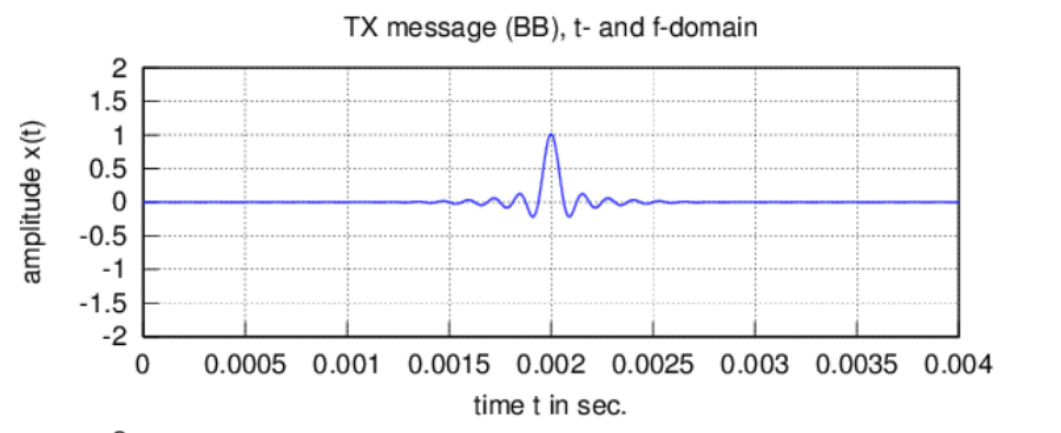
\includegraphics[height=3cm]{./img/mod_einzel_t.png}} ~
	\subfloat[f-domain]{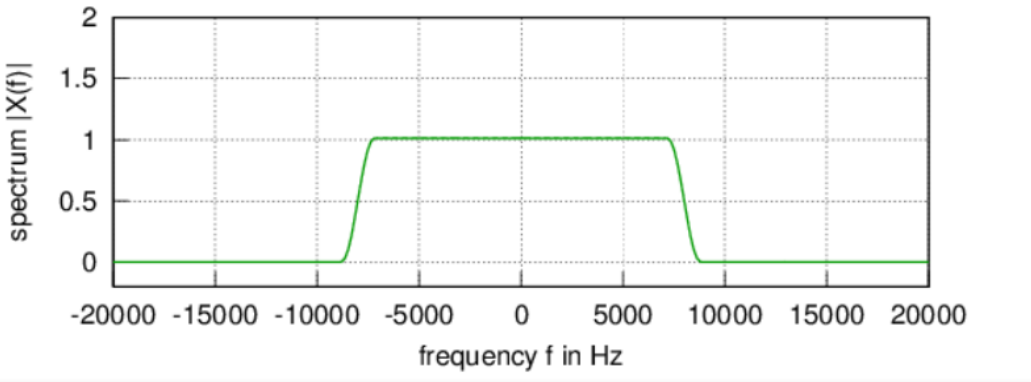
\includegraphics[height=3cm]{./img/mod_einzel_f.png}}
	\caption{Einzelimpuls \protect\cite{NT2}}
\end{figure}

\subsection{Amplitudenmodulation (AM)}
\formTab{Träger}{c(t) = \cos(w_0 t + \varphi_0)}
\formTab{Signal im Passband}{u(t) = \alpha_A \cdot x(t) \cdot c(t) = \alpha_A \cdot x(t) \cdot \cos(w_0 t + \varphi_0) \formTnQQQ = \Re \lbrace \underbrace{x_A \cdot x(t)}_{\text{kompl. Hüllkurve}} \cdot e^{j \varphi_0} \cdot e^{j w_0 t} \rbrace \formTnQQQ = \Re\lbrace x(t) \cdot e^{j w_0 t}\rbrace \quad \text{(für }\varphi = 0 \text{ und  } \alpha_A = 1 \text{)}}
Mit \eqref{eq:fourier_corr_am_1} erhält man durch nutzung der eulerschen Formel
\begin{equation}
	U(w) = \alpha_A \frac{1}{2}\left[X(w+w_0) + X(w-w_0)\right]
\end{equation}

\formTab{Signal mit Offset}{u(t) = \left( x(t) + A_{off} \right) \cdot \cos(w_0 t) \formTnQ = \left( x(t) + A_{off} \right) \left[\frac{1}{2} \cdot e^{j w_0 t} + \frac{1}{2} \cdot e^{-j w_0 t} \right]}
Mit \eqref{eq:fourier_corr_am_off} folgt
\begin{equation}
	x(t) + A_{off} \quad \laplace \quad X(w) + 2\pi A_{off} \delta(w)
\end{equation}

\subsubsection{Frequenzmultiplex}
\formTab{Fourier Identität}{u(t) = \sum\limits_{i=1}^N u_i(t) \quad\laplace\quad U(f) = \sum\limits_{i=1}^N U_i(f)}
\formTab{Kanalraster (bei $\Delta f = const$)}{\Delta f = f_{i+1} - f_i}

\subsubsection{Kohärente Demodulation}
\formTab{Demodulation t-domain}{y(t) = u(t) \cdot \cos(\omega_0 t + \psi) \cdot \beta \formTnQ = u(t) \cdot \cos(\omega_0 t + \psi) \cdot K}
\formTab{Demodulation $\omega$ -/f-domain}{Y(\omega) = \frac{1}{2}X(\omega) \cdot \cos(\psi) \formTn  + \underbrace{\frac{1}{2} X(\omega - 2 \omega_0) \frac{1}{2} \cdot e^{j \psi} + \frac{1}{2} X(\omega + 2 \omega_0) \frac{1}{2} \cdot e^{-j \psi}}_{\text{wird herausgefiltert}}}
\formTab{Typische Normierung}{\alpha_A = \beta = \sqrt{2} \Rightarrow \frac{\alpha_K \beta}{2}=1}
\formTab{Tiefpass Filtereigenschaft}{f_{TP,max} = f_{LP,max} = f_{max,LP} 
\formTnQ f_{max} < f_{max,LP} < 2 f_0 - f_{max}}
\formTab{Orthogonalitätsbedingung}{\psi \neq \frac{\pi}{2} + n \cdot \pi \quad ,\; n \in \Z \quad \text{sonst } v(\omega) = 0} 
\formTab{Identität}{V(\omega) = \frac{1}{2} X(\omega) \cdot \cos(\psi) \quad \formTnQ \laplace \quad v(t) = \frac{1}{2}x(t) \cdot \cos(\psi)}

\subsubsection{Inkohärente Demodulation}
\formTab{Demodulation t-domain}{z(t) = \left[ A_{off} + a(t) \right] \cdot \cos(w_0 t), \; A_{off} + a(t) \overset{!}{>} 0}

\subsection{Quadraturamplitudenmodulation}
Bei der QAM wählt man $x(t) \in \C$ so, dass $X(f)$ asymmetrisch wird und damit die Redundanz der Seitenbänder verschwindet. Es wird ein zusätzlicher Träger der orthogonal zum $\cos$-Träger steht verwendet. Dadurch beeinflussen sich beide Träger nicht.
\formTab{QAM}{u(t) = \alpha_A \left[ x_1(t) \cdot \cos(\omega_0 t) - x_2(t) \cdot \cos(\omega_0 t)\right]} 
Es gilt:
\begin{flalign}
	x(t) = x_{re}(t) + j x_{im}(t) &= x_1(t) + j x_2(t) = x_I (t) + j x_Q(t) + x_N (t) + j x_Q (t) \nonumber \\
	\Rightarrow u(t) &= \Re \lbrace \alpha_A x(t) \cdot e^{j \omega_0 t]} \nonumber \\
	&= \Re \lbrace \alpha_A (x_1 (t) + j x_2 (t)) (\cos(\omega_0 t) + j \cdot \sin(\omega_0 t)) \rbrace \\
	\overset{\alpha_A = 1}{\Rightarrow} u(t) &= x_1(t) \cdot \cos(\omega_0 t) - x_2 (t) \cdot \sin(\omega_0 t)
\end{flalign}
Im Spektrum ergibt sich folglich
\begin{align}
	u(t) &= \Re \left\lbrace \alpha_A x(t) \cdot e^{j \omega_0 t} \right\rbrace \overset{\alpha_A = \sqrt{2}}{=} \frac{\sqrt{2}}{2} \big( x(t) \cdot e^{j \omega_0 t} + \left(x(t) \cdot e^{j \omega_0 t} \right)^* \big) \nonumber\\
	\Rightarrow u(t) \quad &\laplace \quad U(\omega) = \frac{\sqrt{2}}{2} \left( X(\omega - \omega_0) + X^*(-\omega - \omega_0)\right)
\end{align}

\formTab{Demodulation}{v(t) = \beta \cdot u(t) \cdot e^{-j \omega_0 t}}

\subsection{Digitale QAM}
\formTab{Komplexes Symbol}{s_k = s_{k,I} + j s_{k,Q} \quad ,\; s_k \in \frac{1}{\sqrt{2}} \lbrace \pm 1 \pm j \rbrace }
\formTab{Basisbandsignal}{x(t) = \sum\limits_{k=0}^{K-1} s_k g(t-T_s) \quad ,\; T = T_s}
\formTab{Symbolrate}{R_s = \frac{1}{T_s}}
\formTab{Übertragene Bits pro Symbol}{M_b = \ld (M)}
\formTab{Bitrate}{R_b = M_b R_s}

\formTab{Bandbreite (bei Brickstone Impuls)}{B = R_s}
\formTab{Logarithmische Darstellung}{X(f) |_{dB} = 10 \log(X^2(f))}
Das komplexe Basisbandsignal erhält man mit
\begin{align}
	x(t) &= \sum\limits_{k=0}^{K-1} s_k \; g(T-kT_s) = \sum\limits_{k=0}^{K-1} (s_{k,re} + j \; s_{k,im})\;g(t-kT_s) \nonumber\\
	 &= \underbrace{\sum\limits_{k=0}^{K-1} s_{k,re} \; g(t-kT_s)}_{I \in \R} + j\underbrace{\sum\limits_{k=0}^{K-1} s_{k,im}\;  g(t-kT_s)}_{Q \in \R} \quad \in \C
\end{align}

\subsection{Bandbreite für verschiedene $s_k$}
\formTab{Basisbandlage für reelle $s_k$}{B = \frac{1}{2} \; R_s = f_{max}}
\formTab{Basisbandlage für komplexe $s_k$}{B =R_s = 2\cdot f_{max}}
\formTab{Passband für reelle und komplexe $s_k$}{B = R_s =2\cdot f_{max}}

\subsection{Komplexer AWGN Kanal}
\formTab{Kapazität}{C_{AWGN,komplex}(SNR) = 2 \cdot C_{AWGN,reell} (SNR) \formTnQQQ  = \ld (1+SNR)}
\formTab{Rauschleistungsdichte}{N_0 = 2 \sigma^2}
\formTab{Signal-Rausch Abstand}{SNR = \frac{E_s}{N_0}}